\section{Tests at Statkraft's power plant}
\begin{frame}
	\frametitle{Motivation}
	\begin{itemize}
		\item Test the method on more real datasets.
		\item Demonstrate that the method can detect parameter changes.
	\end{itemize}
\end{frame}
\begin{frame}
	\frametitle{Power plant location}
	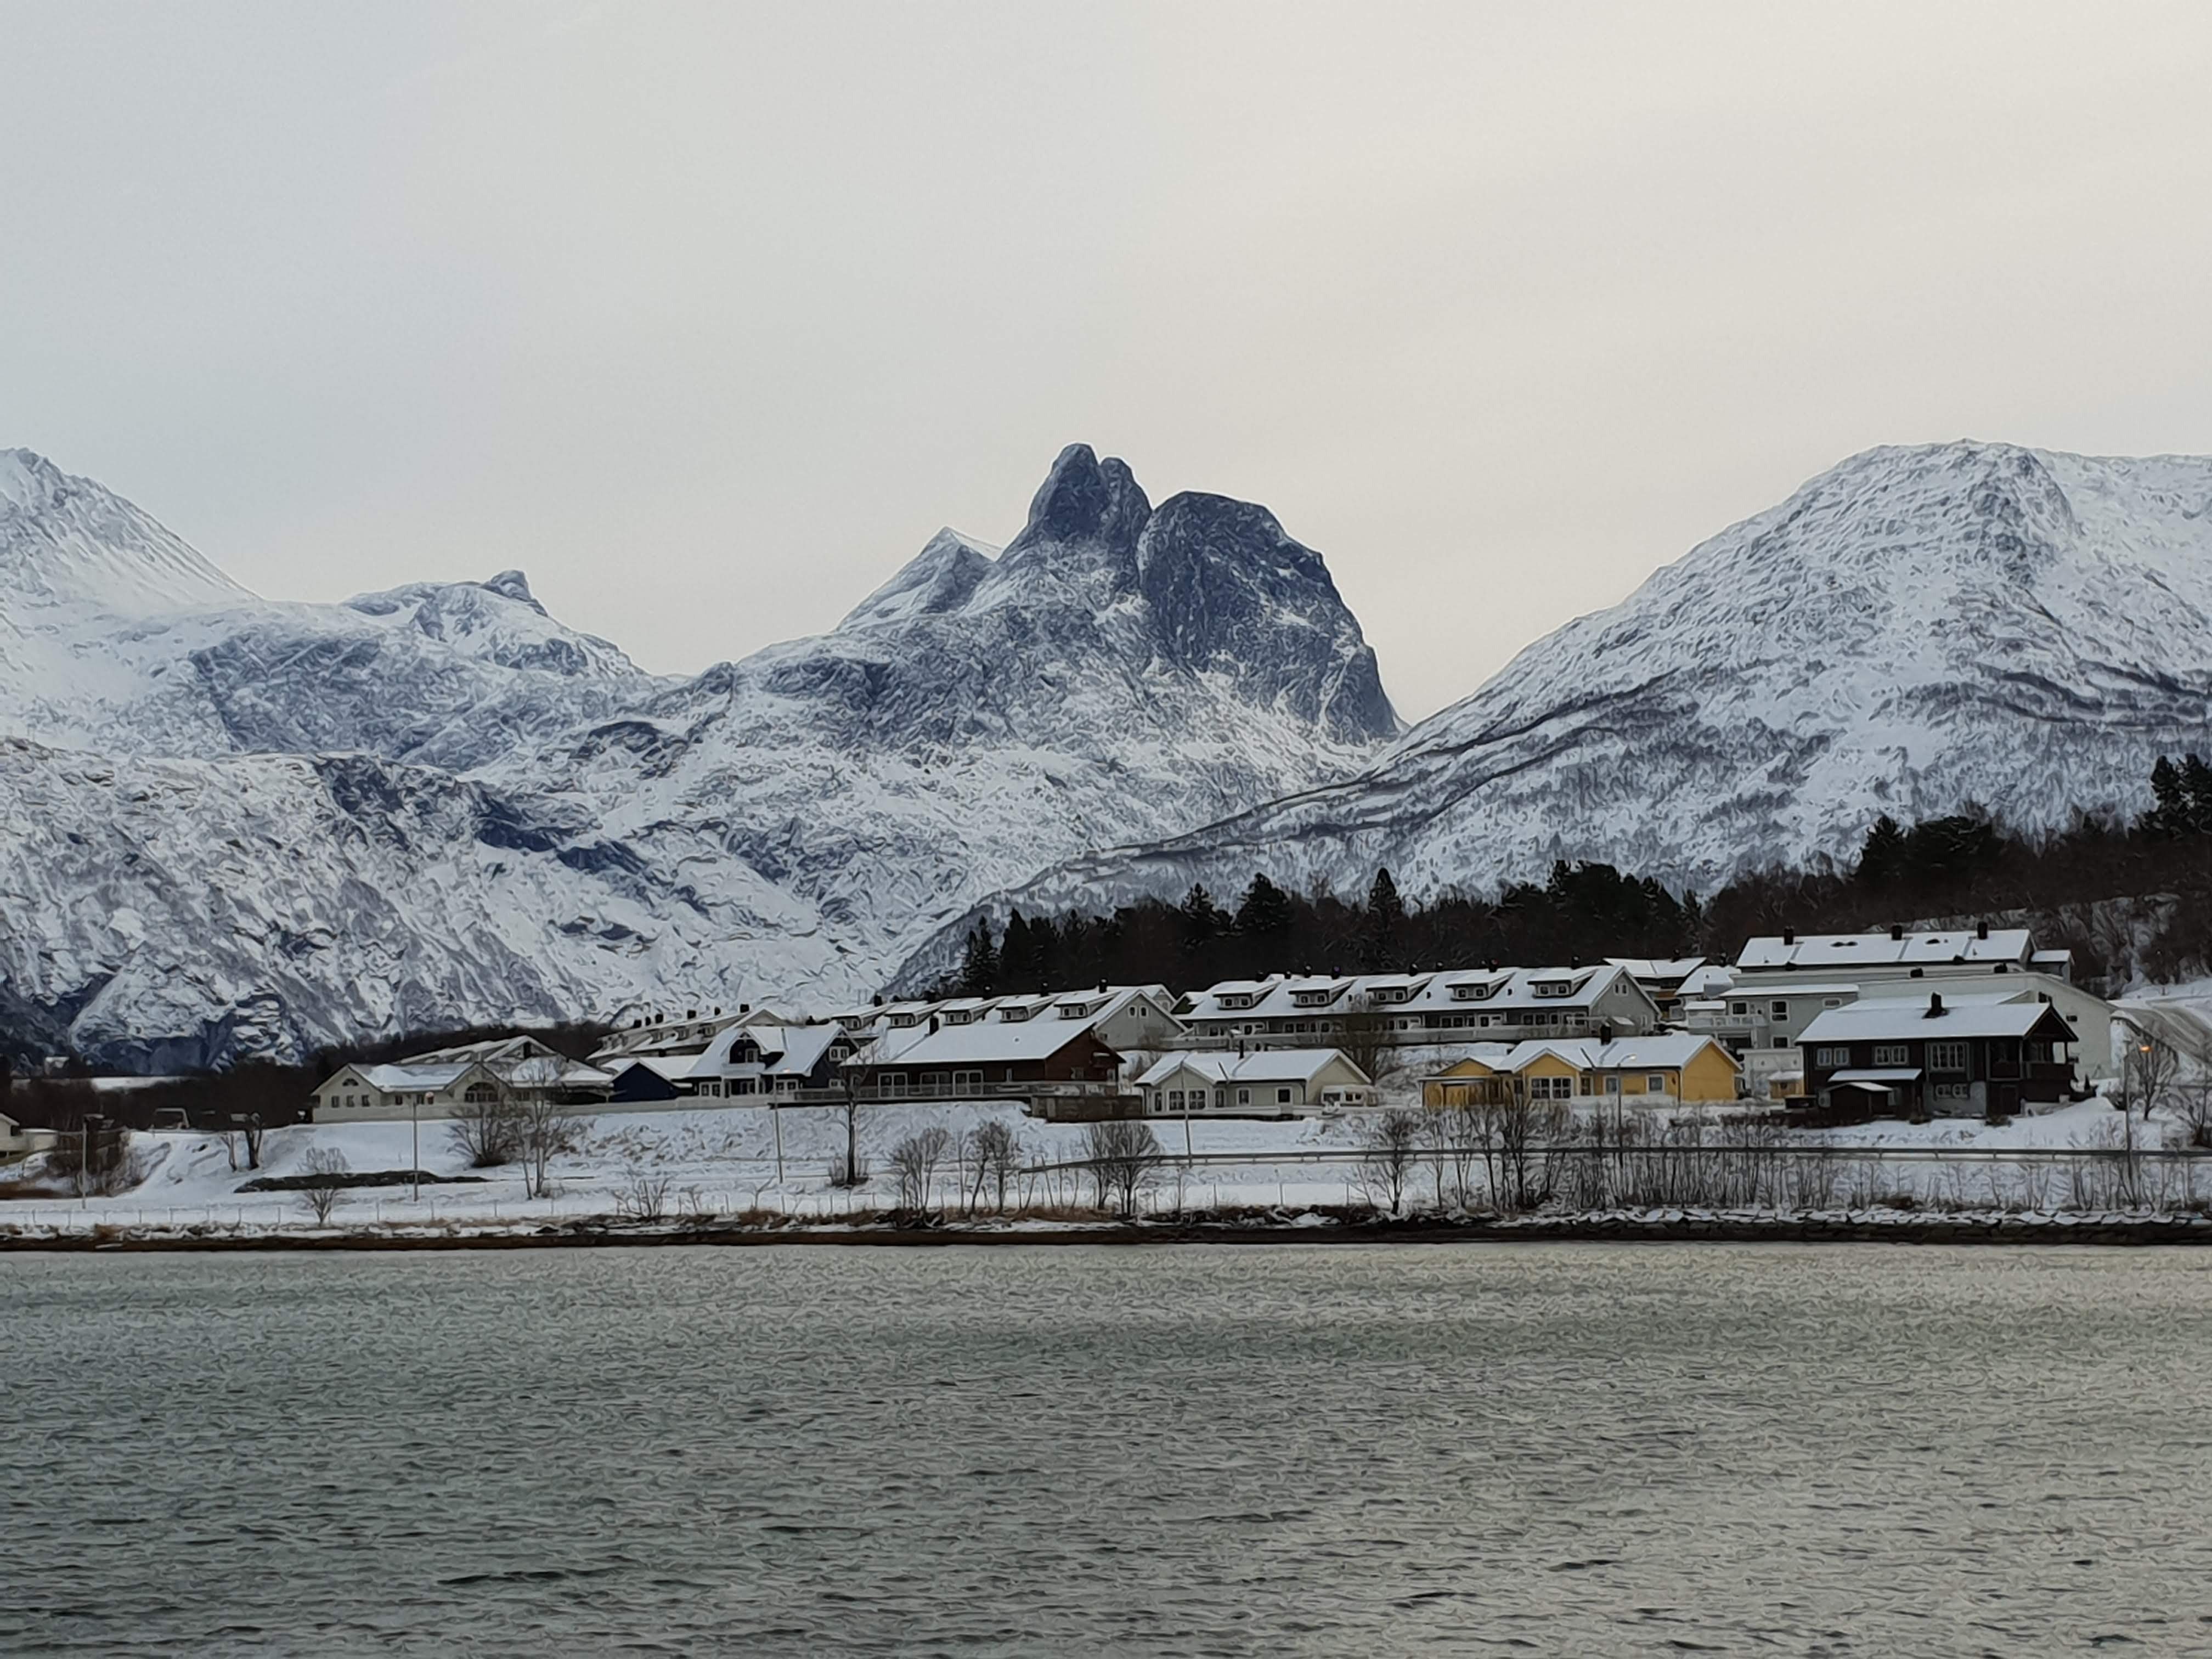
\includegraphics[width=\textwidth]{./pictures/romsdalshorn.jpg}
\end{frame}
\begin{frame}
	\frametitle{Getting data from the control system}
	\begin{columns}
		\begin{column}{0.3\textwidth}
			\begin{itemize}
				\item Collected Electric power $\Delta P_e$
				\item and power system frequency $\Delta f$.
			\end{itemize}
		\end{column}
		\begin{column}{0.7\textwidth}
			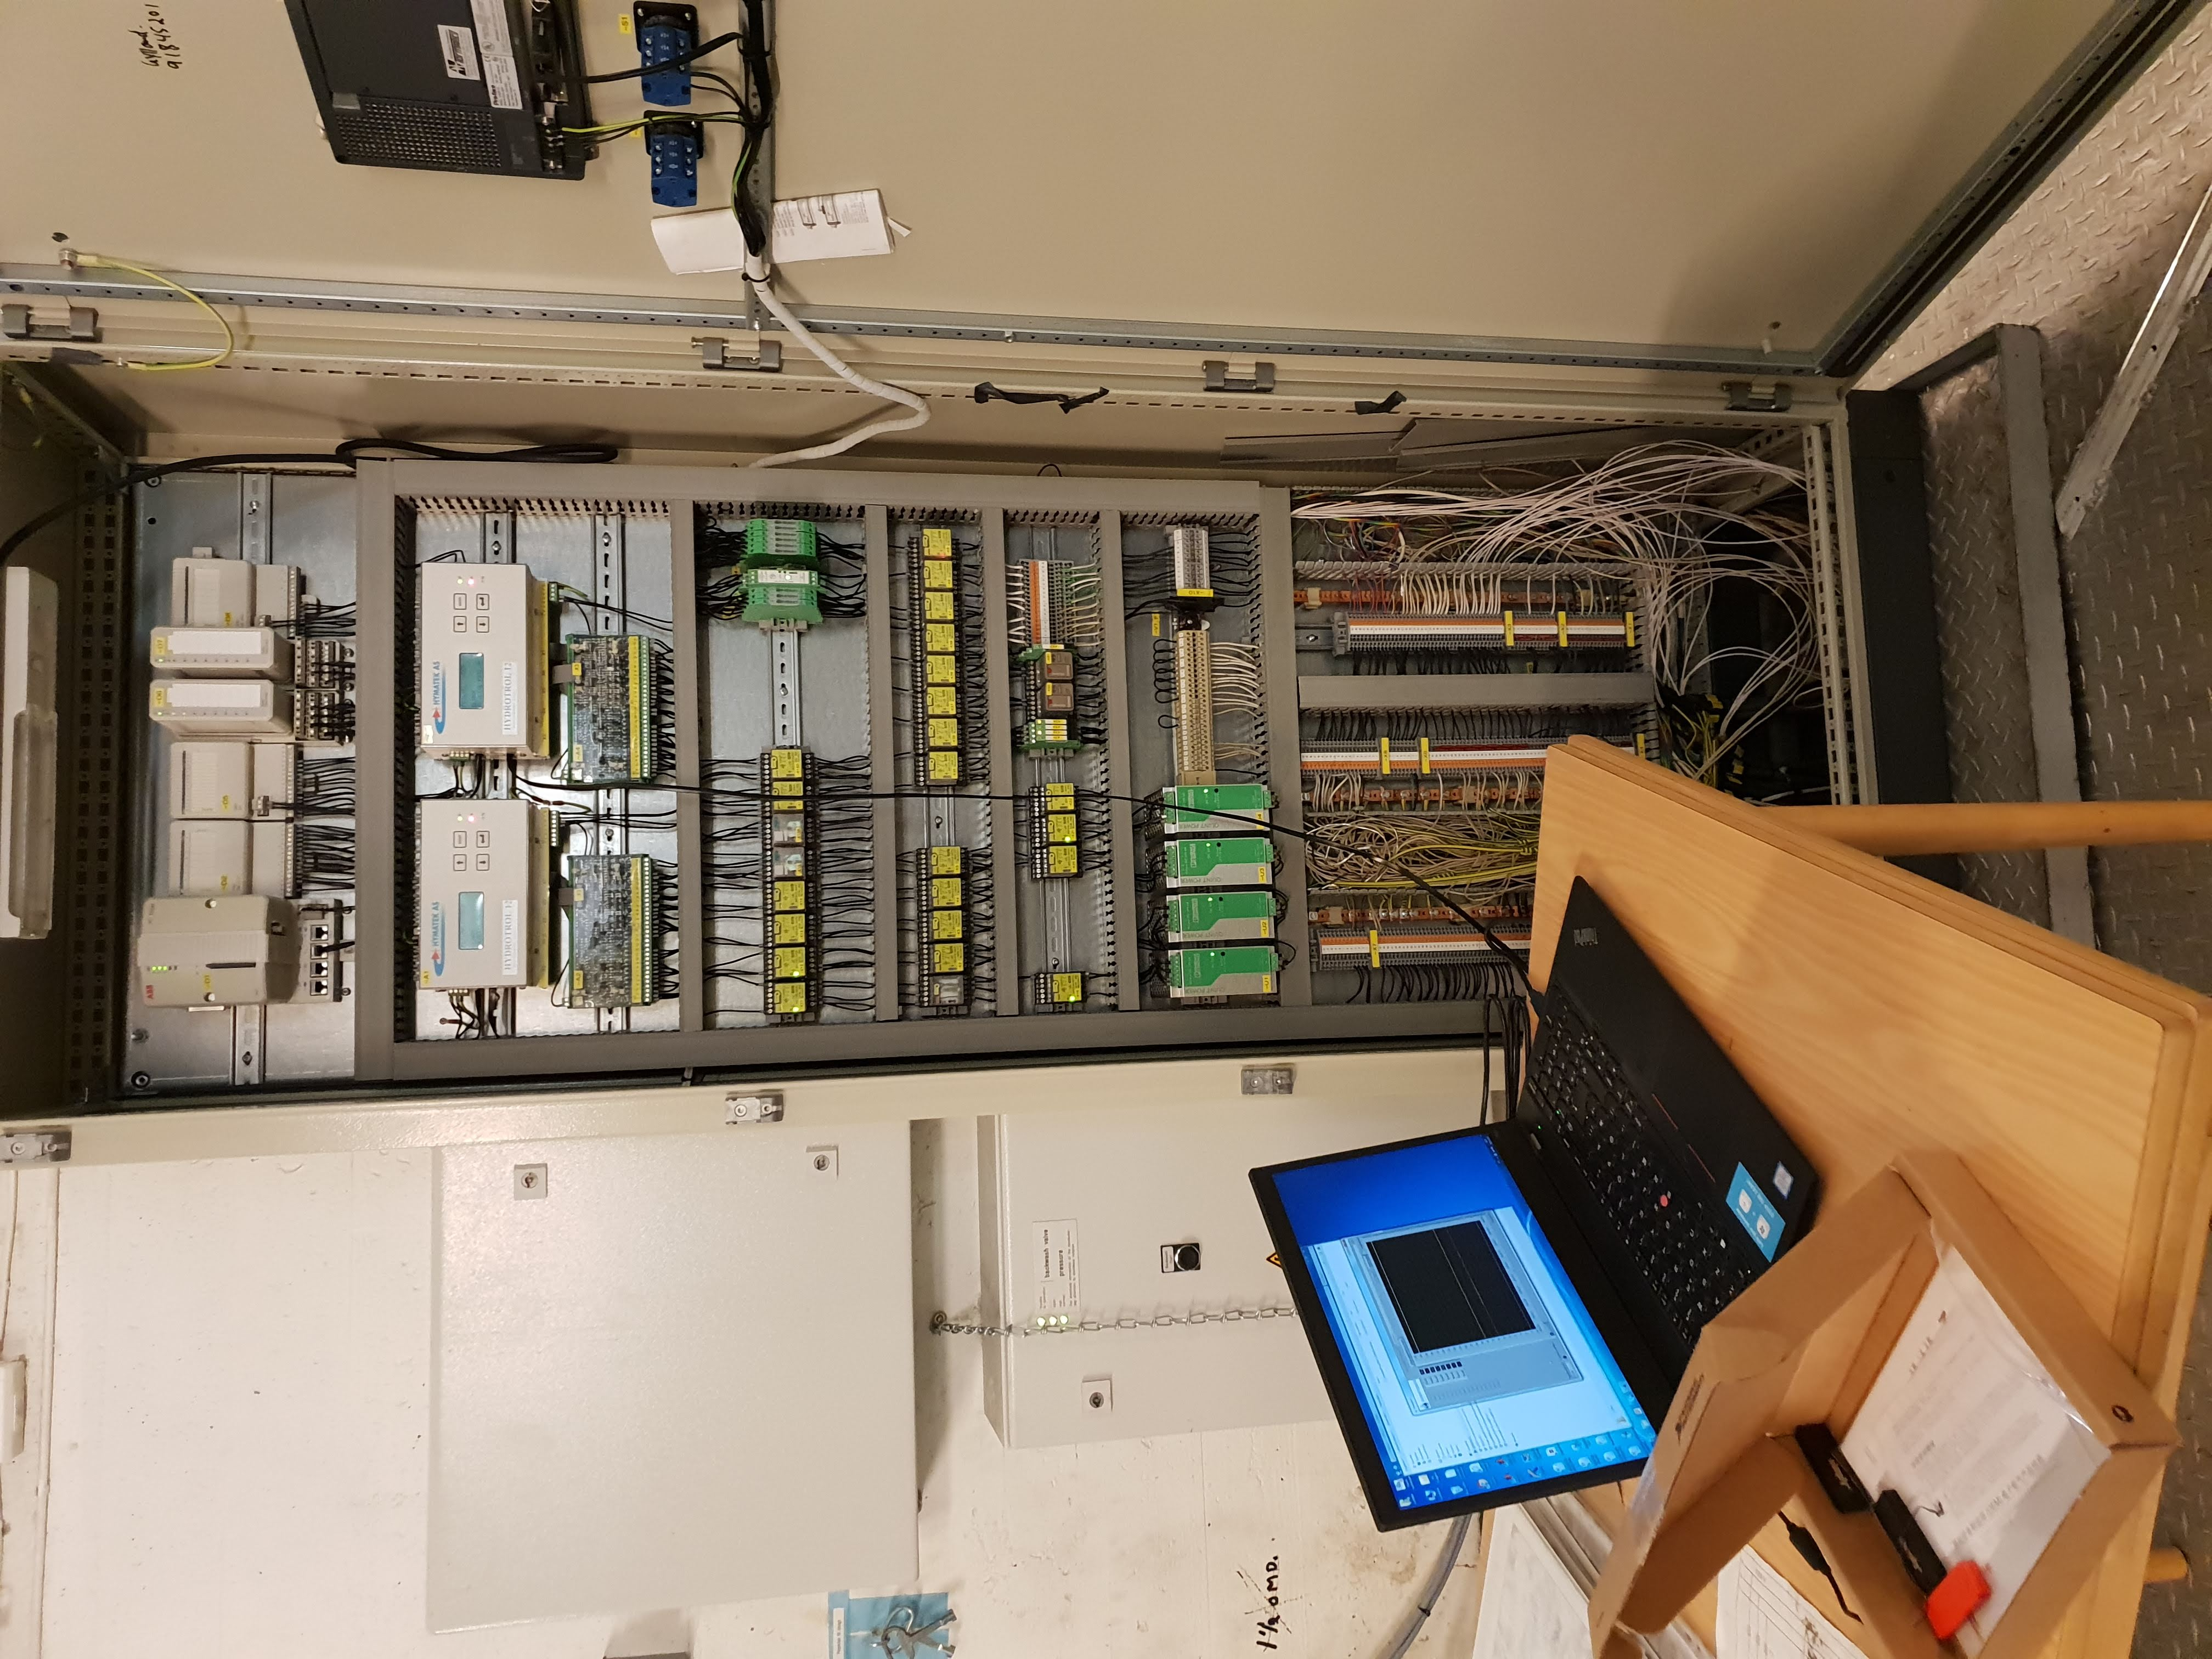
\includegraphics[angle=-90, origin= c, height=\textheight]{./pictures/hymatek.jpg}
		\end{column}
	\end{columns}
\end{frame}
\begin{frame}
	\frametitle{Measurement transformer}
	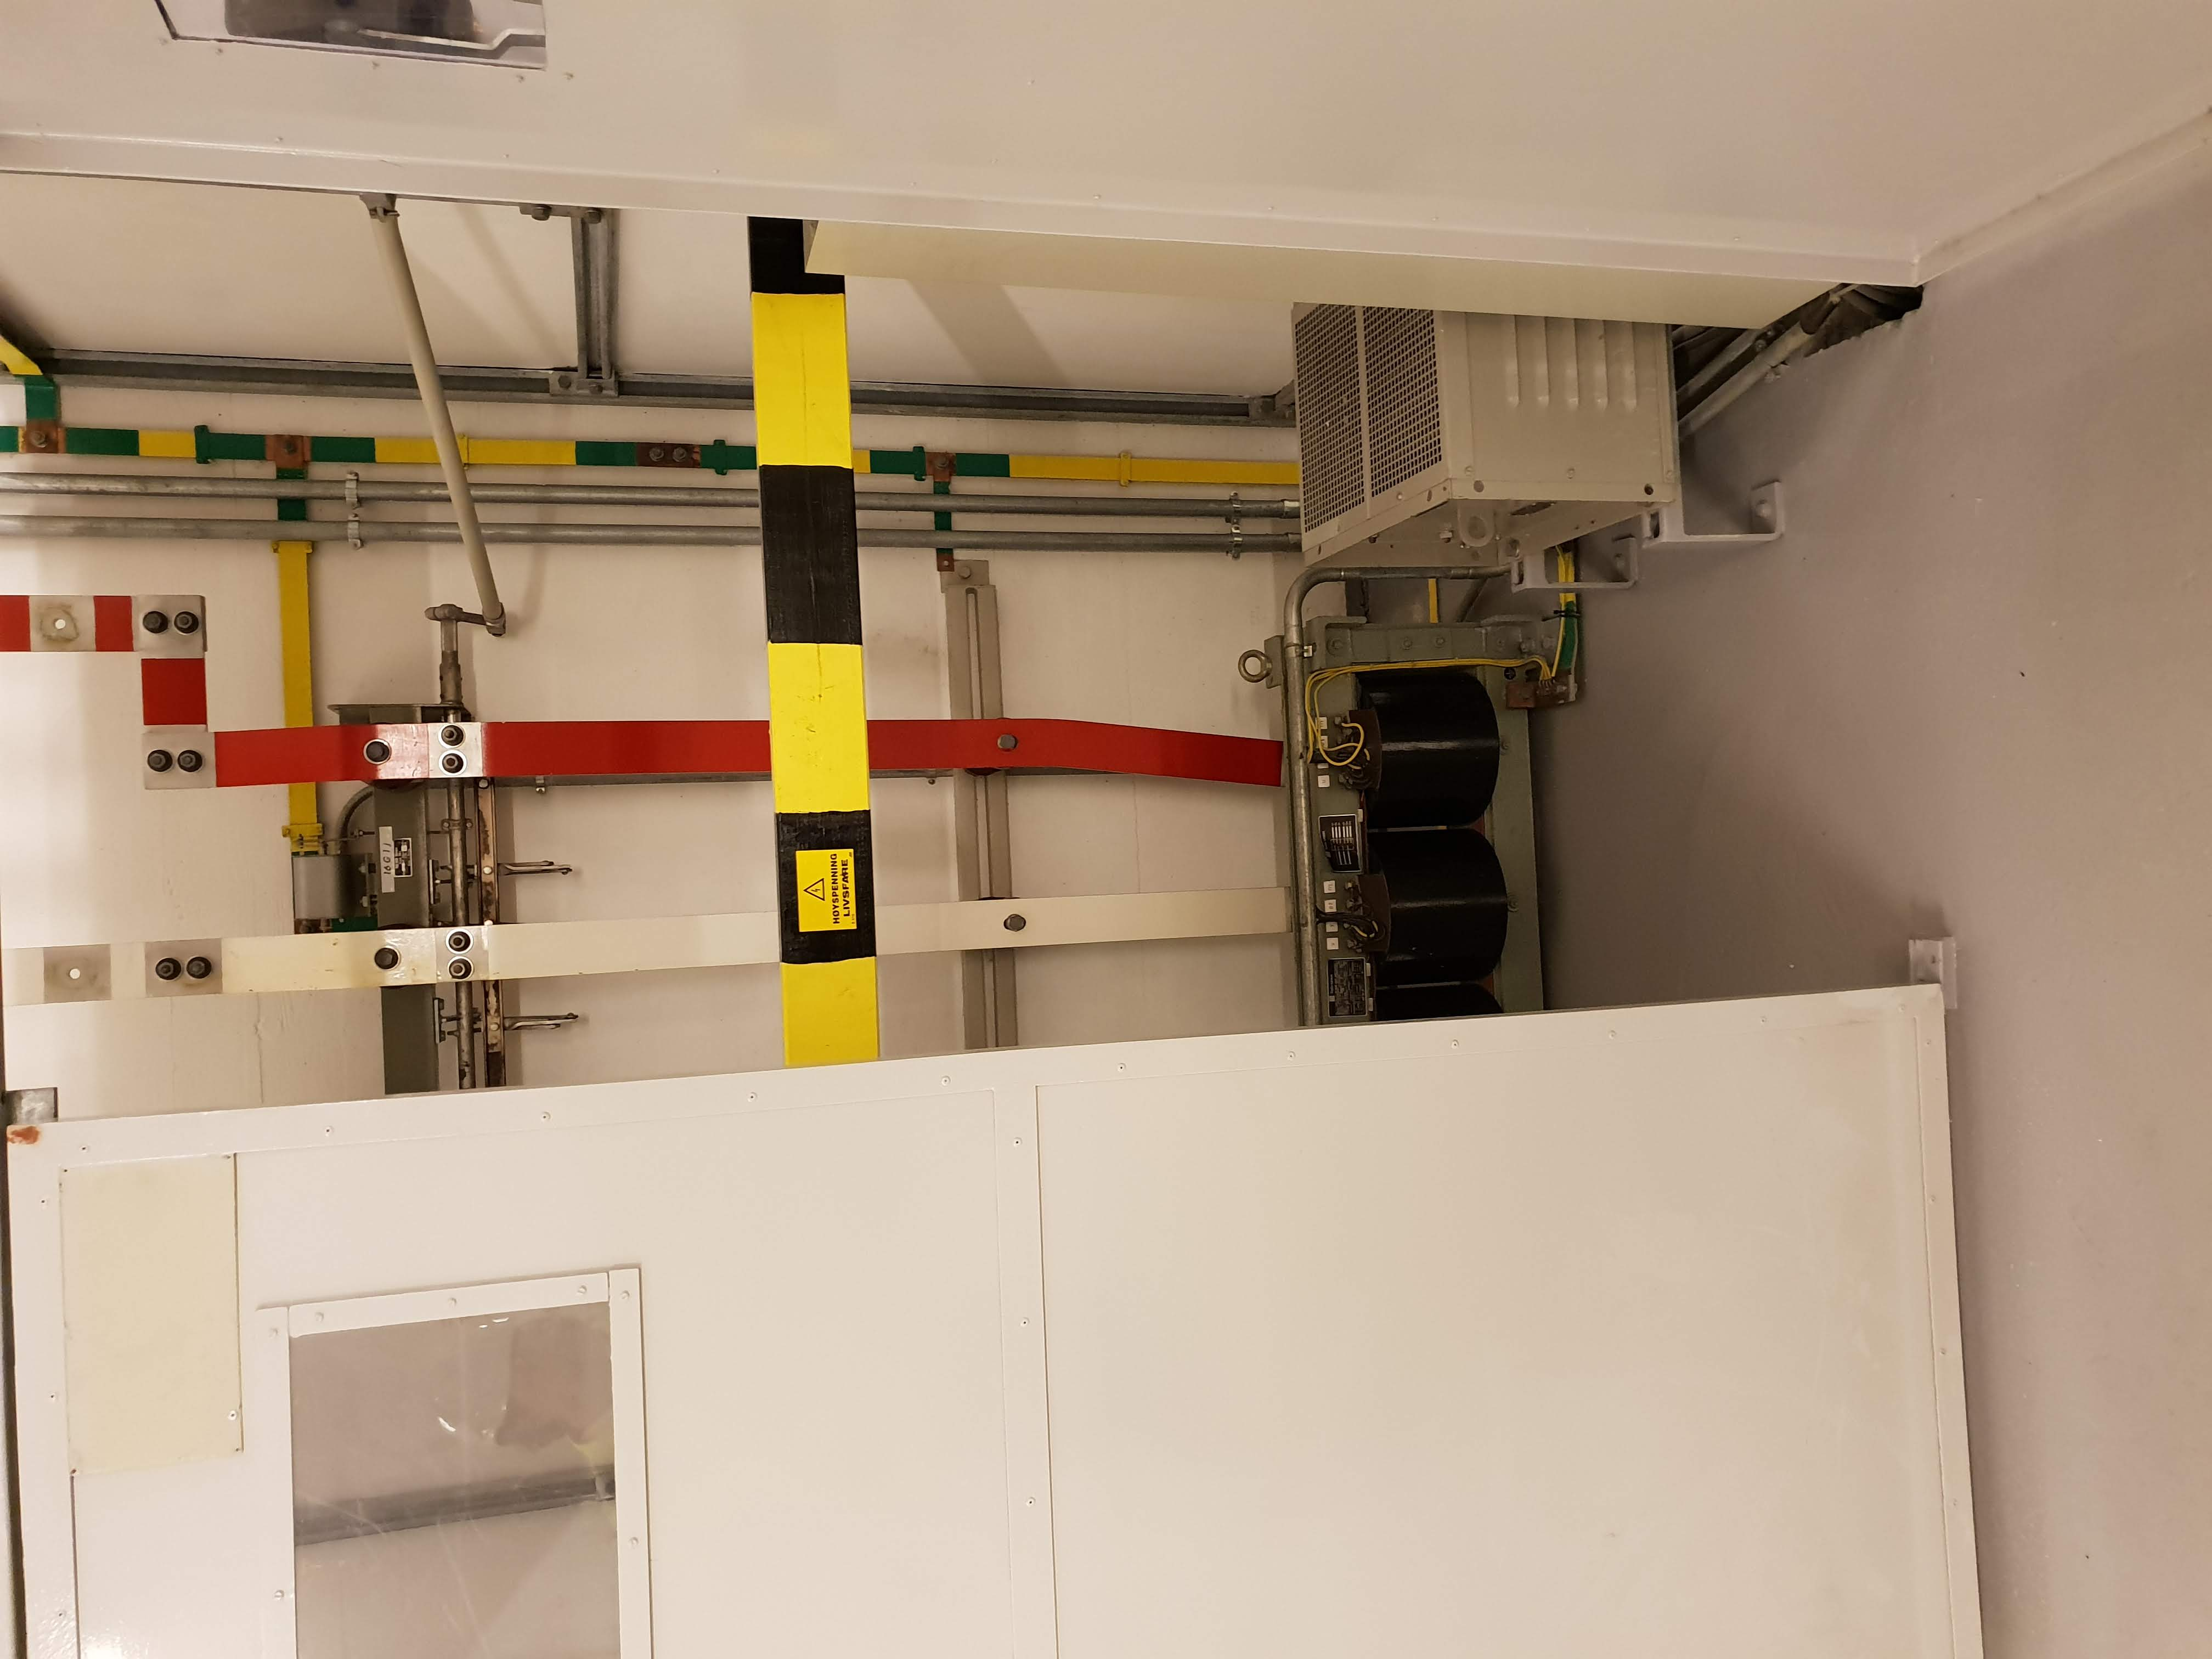
\includegraphics[angle=-90, origin=c, height=\textheight]{./pictures/trafo.jpg}
\end{frame}
\begin{frame}
	\frametitle{Example of dataset}
	\includegraphics[width=\textwidth]{./pictures/Grytten_signals.tikz}
\end{frame}
\begin{frame}
	\frametitle{Detecting a new tuning}
	\begin{columns}
		\begin{column}{0.65\textwidth}
			\includegraphics[width=\textwidth]{./pictures/Grytten_R_5.tikz}
		\end{column}
		\begin{column}{0.35\textwidth}
			\begin{equation*}
				G_1(s) = \frac{G_{J}}{1+G_p(s)G_J(s)}
			\end{equation*}
		\end{column}
	\end{columns}
	\includegraphics{./pictures/sys_G1.tikz}
\end{frame}	
\begin{frame}
	\frametitle{Detecting droop changes}
	\begin{columns}
		\begin{column}{0.65\textwidth}
			\includegraphics[width=\textwidth]{./pictures/Grytten_new_PID.tikz}
		\end{column}
		\begin{column}{0.35\textwidth}
			\begin{equation*}
				G_1(s) = \frac{G_{J}}{1+G_p(s)G_J(s)}
			\end{equation*}
		\end{column}
	\end{columns}
	\includegraphics{./pictures/sys_G1.tikz}
\end{frame}	
